\section{\secState{R}Comparison to Other Methods}\label{s:OtherMethodsComparison}
\noindent The \emph{testing} (sec. \ref{s:testPlan}) is strongly \emph{capability} oriented, some performance testing regrading computational load (sec. \ref{s:ComputaitonFootprint}) is on the place. The advantages of our approach regarding scalability are outlined in (sec. \ref{s:conclusionScalability}).

This section summarizes the results achieved by one of the master students \cite{hrdlik2018}. Who compares other avoidance methods concerning performance. The  \emph{conservative }vector field avoidance \cite{borenstein1991vector} and \emph{adaptive} potential field \cite{koren1991potential} methods are compared to our approach (sec. \ref{s:conservativeComparison}).

\subsection{\secState{R}Conservative and Adaptive Method Comparison}\label{s:conservativeComparison}
\paragraph{Testing scenario:} The testing scenario is similar to \emph{building avoidance} (sec. \ref{s:testBuildingAvoidance}), using the default framework testing configuration (sec. \ref{sec:testingConfiguration}). The \emph{reach set approximation} used is a \emph{combination of harmonic and chaotic} (fig. \ref{fig:combinedReachSetApproximation}) filling the role for \emph{navigation/avoidance} in non controlled airspace. The \emph{mission} is given by waypoints defined in (tab. \ref{tab:missionSetupForPErformanceTest}), the UAS is starting at $\mathscr{WP}_1$.

\begin{table}[H]
	\centering
	\begin{tabular}{c|c||c|c|c|c|c}
		\multicolumn{2}{c||}{Position} & \multicolumn{4}{c}{Waypoints} \\\hline
		$[x,y,z]$     & $[\theta,\varpi,\psi]$           & $\mathscr{WP}_1$   & $\mathscr{WP}_2$   & $\mathscr{WP}_3$   & $\mathscr{WP}_4$    & $\mathscr{WP}_5$\\\hline\hline
		$[0,0,0]^T $       & $[0^\circ,0^\circ,0^\circ]^T$ & $[0,0,0]^T$ & $[20,0,0]^T$       & $[20,20,0]^T$       & $[0,20,0]^T$       & $[0,0,10]^T$       
	\end{tabular}
	\caption{Mission setup for \emph{Performance test} scenario.}
	\label{tab:missionSetupForPErformanceTest}
\end{table}

\noindent The \emph{static obstacle set} (tab. \ref{tab:obstacleSetComparison}) contains three obstacles in the middle of waypoints. The obstacles are balls with uniform radius. The concept of \emph{body} and \emph{safety margin} was not used in this test.

\begin{table}[H]
	\centering
	\begin{tabular}{c|c|c|c}
		\multicolumn{3}{c|}{Obstacle} &  \multirow{2}{*}{Radius}\\\cline{1-3}
		id & position & type  &   \\\hline\hline
		$1$ & $[10,0,0]^T$ & ball  &$2$ \\\hline
		$2$ & $[20,10,0]^T$ & ball & $2$ \\\hline 
		$3$ & $[10,20,0]^T$ & ball  & $2$ 
	 \end{tabular}
	\caption{\emph{Obstacle set} for \emph{Building avoidance} scenario.}
	\label{tab:obstacleSetComparison}
\end{table}

\begin{note}
The z coordinate value of zero does not represent the ground in this test scenario, because some methods do not support ground avoidance like ours. 
\end{note}

\paragraph{Scenario example:} The \emph{scenario} was run for the following approaches:
\begin{enumerate}
    \item \emph{Static obstacle avoidance based on reach sets} - implementation \cite{hrdlik2018} of \cite{gomola2017obstacle}, using own framework.
    
    \item \emph{Conservative } - vector field avoidance \cite{borenstein1991vector}, adapted implementation \cite{hrdlik2018}.
    
    \item \emph{Adaptive} - potential field \cite{koren1991potential}, adapted implementation \cite{hrdlik2018}.
\end{enumerate}

\noindent The example of the testing framework developed by my student is shown in (fig. \ref{fig:avoidancePerformanceScenarioHrdlik}). The \emph{obstacles} are big red balls consisting from smaller red balls, representing LiDAR sensor hit zones. The \emph{UAS} sensing range is represented as an area outlined with a black dashed line. The waypoints are marked as green squares. The flew trajectory is represented as blue line. The \emph{planned trajectories} (red line) for decision frames (magenta circle) which are not executed are also shown.

\begin{figure}[H]
    \centering
    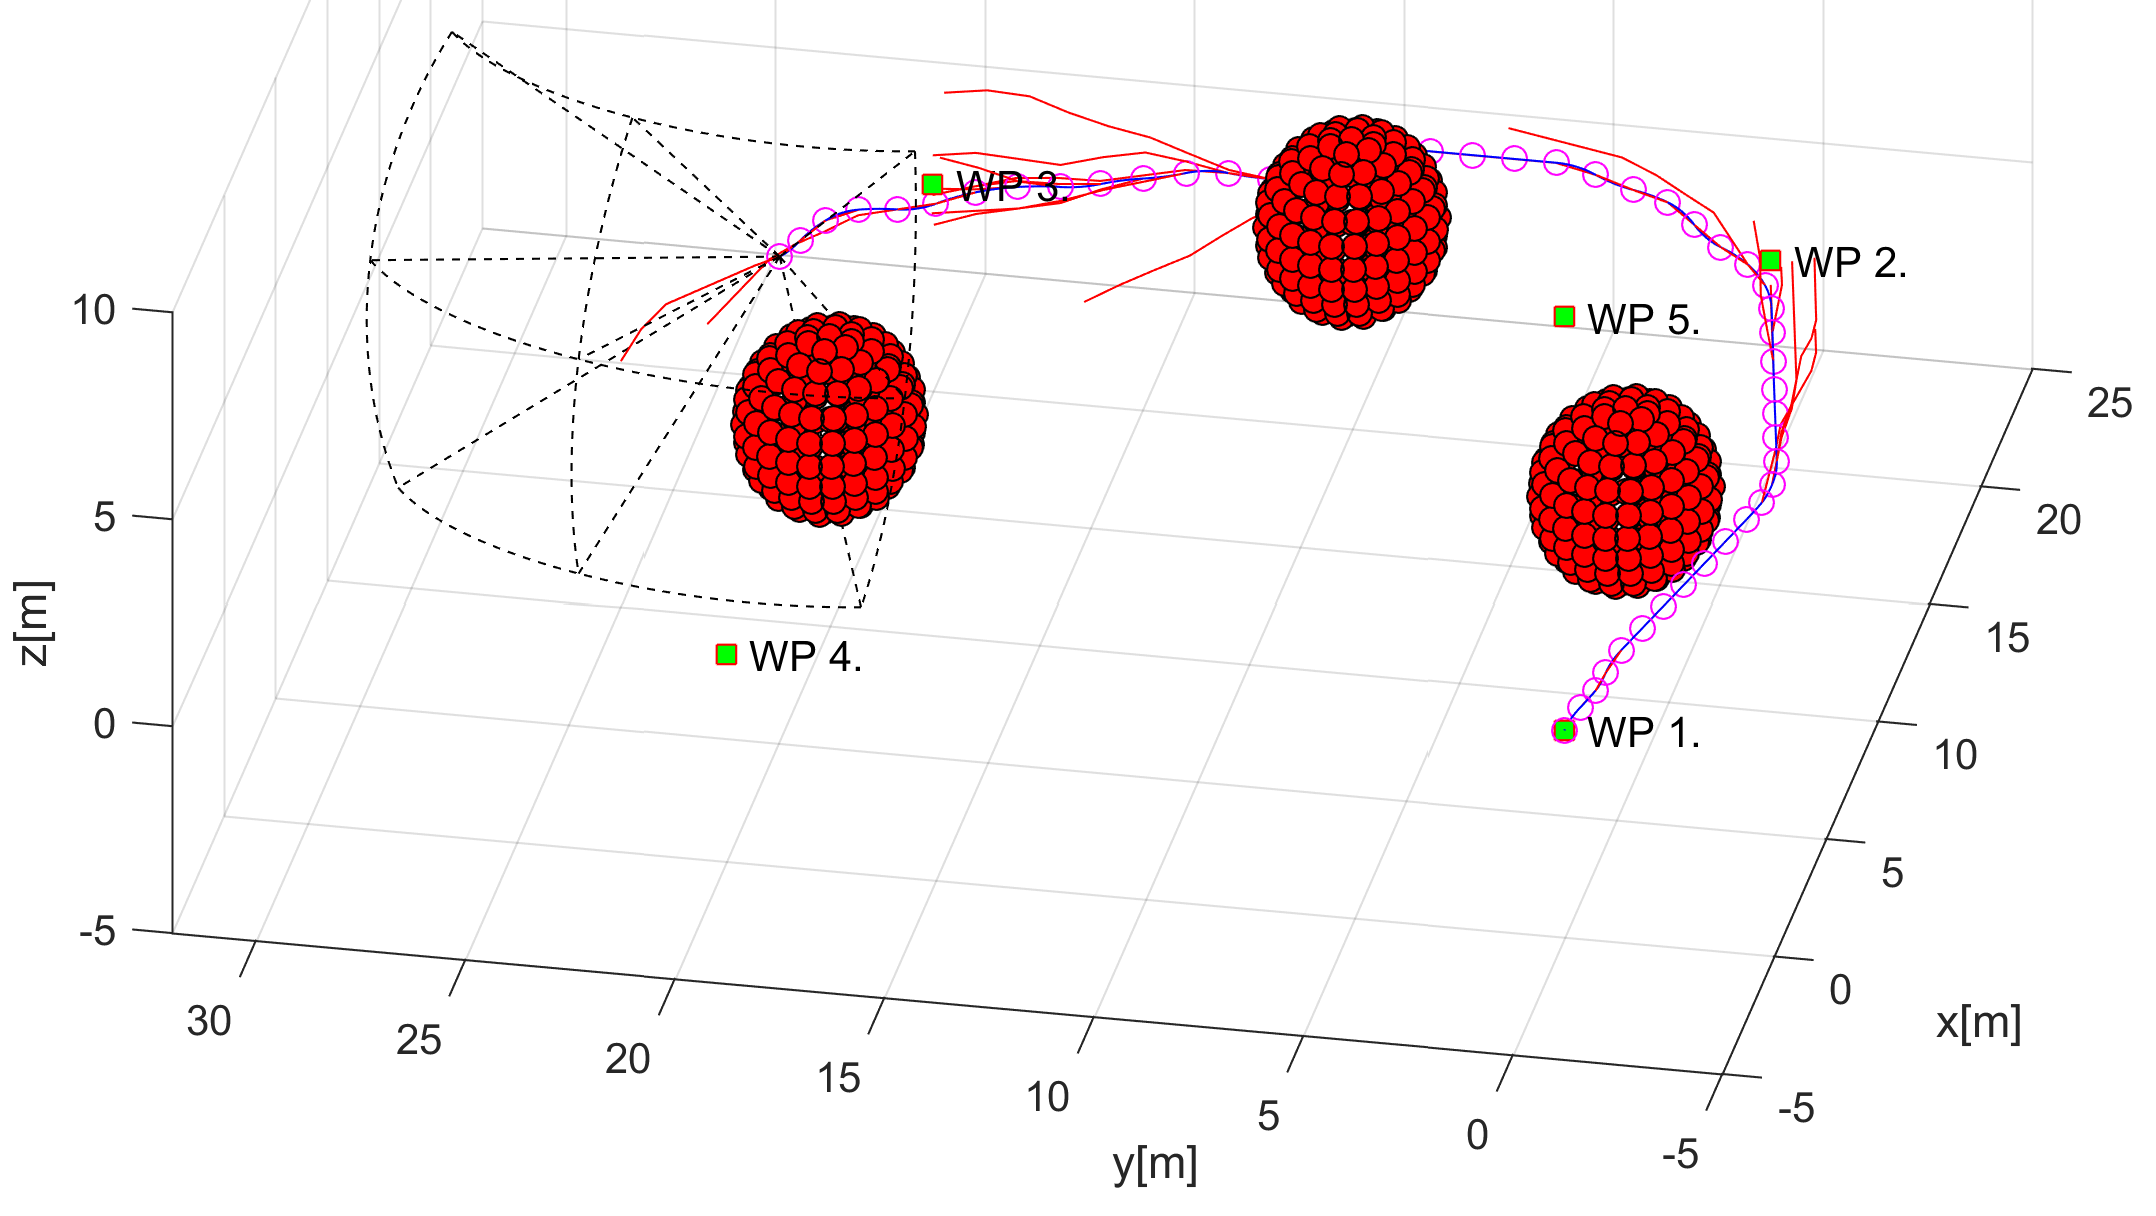
\includegraphics[width=0.7\linewidth]{\FIGDIR/C001TestingScenario} 
    \caption{A testing scenario for method performance comparison \cite{hrdlik2018}.}
    \label{fig:avoidancePerformanceScenarioHrdlik}
\end{figure}

\paragraph{Conservative Method Performance Margin:} The \emph{principle} of the conservative method is like follows: \emph{Every time there must be a place to turn without the context}. The conservative method performance margin was estimated by \cite{hrdlik2018} like follow:

\begin{equation*}
    conservative_{margin} = 2 \times turning Radius +3 \times uas Radius
\end{equation*}

\noindent Using parameters from our testing configuration (sec. \ref{sec:testingConfiguration}) where the turning radius is 2 and UAS body radius is 0.6 the theoretical $conservative_{margin}$ is $4.6$.

\paragraph{Conservative Method Performance Margin:} The \emph{principle} of the conservative method is like follows: \emph{Every mass point has a potential equal to its expected mass, those potentials repel each other with proportional force}. The adaptive method performance margin was estimated by \cite{hrdlik2018} like follow:

\begin{equation*}
    adaptive_{margin} = 3\times uas Radius
\end{equation*}

\noindent Using parameters from our testing configuration (sec. \ref{sec:testingConfiguration}) where the UAS body radius is 0.6 the theoretical $adaptive_{margin}$ is $1.8$.

\begin{note}
    The \emph{real conservative and method performance}  was close to \emph{theoretical best performance} \cite{hrdlik2018}.
\end{note}

\paragraph{Distance to Body Margin Evolution:} The performance of an \emph{obstacle avoidance framework based on reach set} for the mission (tab. \ref{tab:missionSetupForPErformanceTest}) is shown in (fig. \ref{fig:crashDistanceEvolution}). The critical margin (crash zone) is 0.6 (UAS body radius) and is denoted as a red dashed line. The \emph{adaptive margin} id 1.8 and its denoted as a yellow dashed line. The \emph{conservative margin} is 4.6 and its denoted as green dashed line. 

The distance to the \emph{body margin} of the UAS center stayed mostly in \emph{adaptive zone} (yellow line) and two times entered into \emph{outperforming zone} (red line). The \emph{outperforming zone} is distance values between:

\begin{equation*}
    critical Margin (0.6) \ge outperforming Zone < adaptive Margin (1.8)   
\end{equation*}

One can say that reach set method outperforms selected conservative and adaptive methods representatives.

\begin{figure}[H]
    \centering
    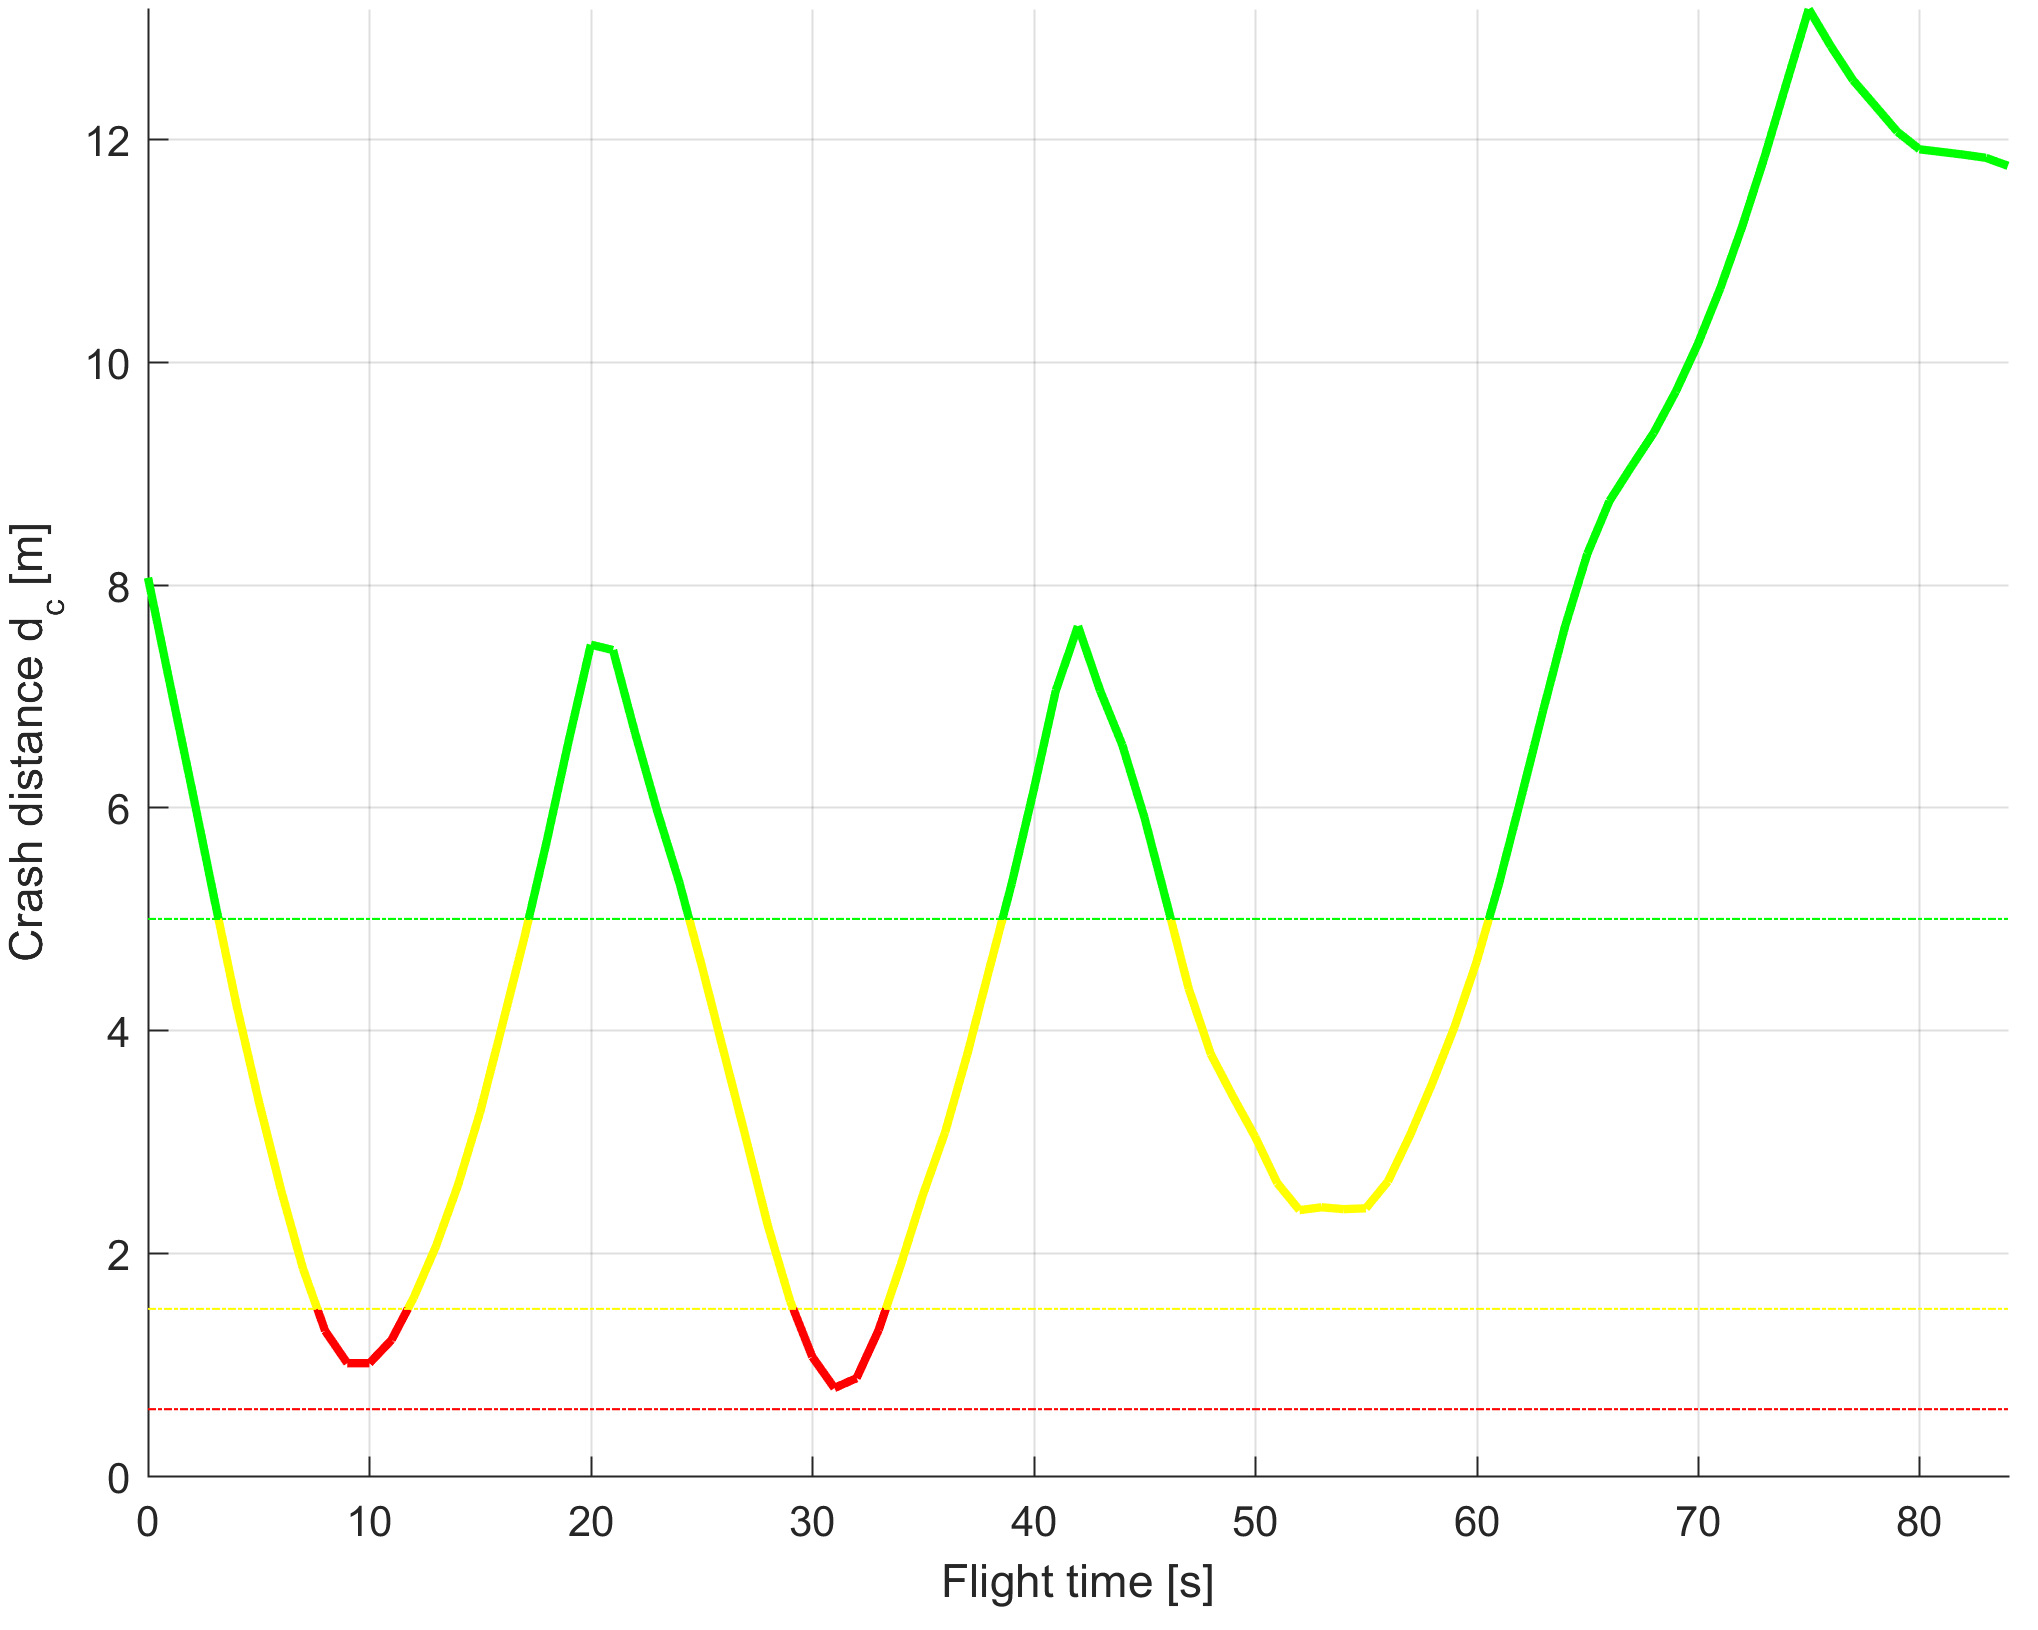
\includegraphics[width=0.7\linewidth]{\FIGDIR/C002CrashDistanceEvolution} 
    \caption{Distance to body margin evolution \cite{hrdlik2018}.}
    \label{fig:crashDistanceEvolution}
\end{figure}

\paragraph{Disclaimer:} Further investigation regarding \emph{cost-effectiveness} is required, the approach needs to be tested in real environment and on the multiple scenarios. The testing concerning approach feasibility have been proven (tab. \ref{tab:testCasesPerformacneEvaluation}).

\subsection{\secState{R}Scalability}\label{s:conclusionScalability}
\noindent The \emph{many methods} do not offer \emph{scalability}. The scalability means that method applies to multiple problems with different scale or there is a sufficient amount of tune-able parameter to make it work in different environments. Many avoidance concepts have hardwired margins. 

The \emph{Detect and Avoid} system must offer scalability to some extent, because of changing regulations and performance criteria on the UAS systems.

\paragraph{Range scalability:} The physical constraints need to be sensed by sensor array in avoidance grid, and the UAS cannot get to close to them. 

\paragraph{Static obstacles:} The body margin or the minimal distance of UAS center to obstacle body is constrained like follow:

\begin{equation*}
    uas Radius < body Margin \le grid Range
\end{equation*}

The \emph{tuning parameter} for static obstacles is \emph{safety margin} is then constrained like follow:

\begin{equation*}
    body Margin < safety Margin \le \infty
\end{equation*}


The constraints for safety margin calculation and some guidelines were outlined in (sec. \ref{s:safetyMarginCalculation}).

\paragraph{Intruders:} The \emph{intruders} (sec. \ref{s:intruders}) are limited by \emph{detection range} and intersection models parameters ranges. 

The \emph{body volume intersection} (sec. \ref{s:bodyvolumeIntersection}) has a following constraint:

\begin{equation*}
    intruder Radius < body Radius \le minimal Detection Range - 2 \times our UAS radius
\end{equation*}

\begin{note}
    The \emph{body radius} does not need to fit exactly on the intruder real body radius; usually, some padding space is added.
\end{note}

The \emph{maneuverability uncertainty intersection} (sec. \ref{s:uncertaintyIntersection}) is tuned through the uncertainty spread on the horizontal and vertical plane. This spread cannot be infinite, and the only limitation is given by implementation:

\begin{equation*}
    \begin{aligned}
        0^\circ & \le&  horizontal Spread &< &90^\circ\\
        0^\circ & \le&  vertical Spread &< &90^\circ
    \end{aligned}
\end{equation*}



\paragraph{Constraints:} The constraints are considered as \emph{airspace restrictions}, \emph{weather zones}, \emph{geo-fencing zones} in this work. The constraints have two implementations \emph{Static constraints} (sec. \ref{s:virtualConstraints}) and \emph{Moving constraints} (sec. \ref{s:MovingVirtualConstraints}). The only real constraint is the detection range; the constraint must be detected before making any impact on \emph{grid}:

\begin{equation*}
    impact(uasPosition,constraintCenter) < detection Range - grid Range
\end{equation*}



